This is one of the main part of \textsl{Neuromuse3}. Indeed, the aim here is to create connections between each \textit{microcolonne} -- or \textit{fanal} -- as \textit{tournois} inside a neuronal AREA as cliques. 

Then, the learning process consists to connect a set of SOM together in order to create an associative memory.

\bigskip

The \textit{macrocolonne} is managed by the class AREA, establishing the connections of each clique from each identified \textit{fanal} involving relationships with incoming and outgoing arcs for each \textit{fanal}. Then, each arc as the key of the hash table of AREA will be associated to a weight.

%add here example or clarity

\bigskip

As seen previously, the method  \glspl{locate-tournoi} gives as result a list of potential  \textit{tournois}, which by cross-checking with the \textit{tournois} of the other \textit{colonnes} -- correlated  in terms of cliques -- allow the (re-)construction\footnote{The (re-)construction must be understood in terms of reminder and invention.} of a sequence according to the user `condition(s)'. 

\smallskip

In the same vein, the method \glspl{locate-clique} allows to retrace clique(s) from partial data. Thus, from this step, the (re-)construction of a sequence which is connected to the reading of \textit{tournois}, is done in a field of arcs and edges according to a deliberate heuristic by consensus and iteration.

\smallskip

The (re-)construction is effective when a learned sequence can be retraced as recollection or retrieving memory or as creation. In all case, this implies modalities defined by the user -- see diagram on figure \ref{fig:mlt2}\footnote{Concerning the diagram of the figure \ref{fig:mlt2}:
\begin{itemize}
\item[$\bullet$]  The constraints or rules allow to limite the field of search, or in other words the constraints aims to reduce the field of possibilities. This can be done with as examples, harmonic rules, a specific scale or whatever. It would be possible to define the `rules' on an interactive way, as a live coding for instance -- involving  in both case the user with its own code --, allowing the adaptability in terms of reaction to the immediate environment.
\item[$\bullet$]  The bayesian inference can play a role for the estimation of a response in terms of probability focusing on the acquis -- that is to say the highest probability.
\item[$\bullet$]  The resolution is done on the filtered probabilities in order to get an optimal solution, which one can be oriented with some a posteriori rule(s) of the user. 
\item[$\bullet$] Note that for now, the user interaction allows to manage the interrelationship between the agent and its environment in terms of affect.
\end{itemize}}.

\bigskip

\begin{figure}[htbp]
\begin{center}
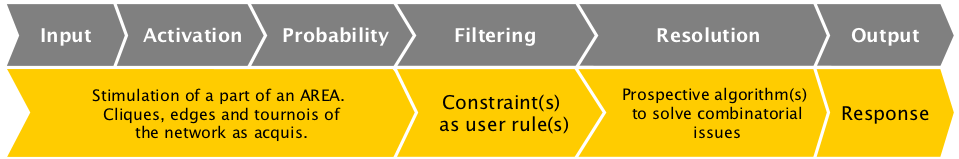
\includegraphics[width=\textwidth]{2551}
\caption{Synoptic diagram of resolution I/O at the AREA level.}
\label{fig:mlt2}
\end{center}
\end{figure}

%\item[$\bullet$]  The valence of a potential response fits within context of  predictability.

%\bigskip
%\newpage
The method \glspl{locate-clique} allows a first estimation of possible clique(s) according to two possible inputs:
\begin{enumerate}
\item isolated node(s): \texttt{((microcolonne\_indice colonne\_indice) …)}
\item ordered node(s): list of \textit{microcolonne} indice(s) and/or wild card ordered according to the soms-list.
\end{enumerate}

All connected  \textit{microcolonnes} to known elements are listed. This is what we observe on the figure \ref{fig:mlt1} with the nodes (4 0) and (1 3), respectively the fifth \textit{fanal} of SOM 1 and the second \textit{fanal} of SOM 4. 
All microcolonnes whose connection number is equal to the number of known elements are collected. These connections are represented in solid lines.

\begin{figure}[htbp]
\begin{center}
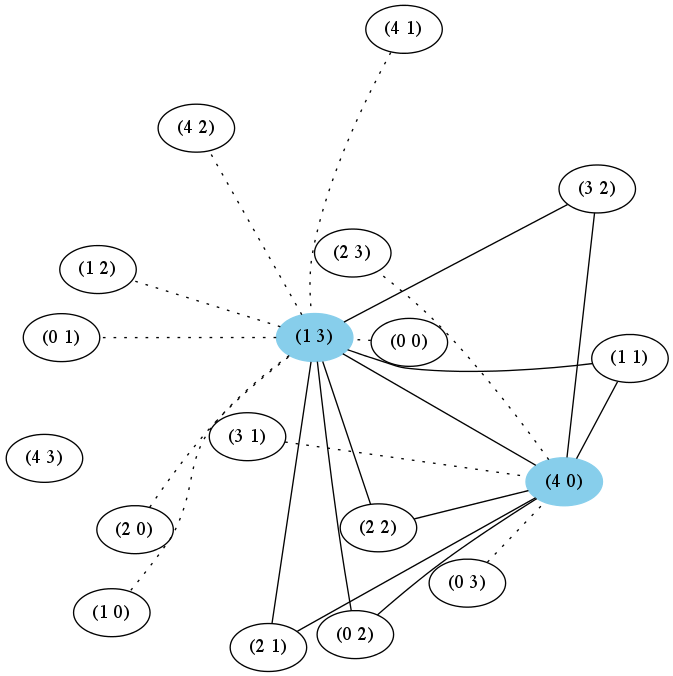
\includegraphics[width=8cm]{2701}
\caption[Cliques estimation on a network AREA (partial view) composed of four SOM of five \textit{fanaux}.]{Cliques estimation on a network AREA (partial view\protect\footnotemark) composed of four SOM of five \textit{fanaux}.}
\label{fig:mlt1}
\end{center}
\end{figure}

\footnotetext{Generated with \color{n3comment}{{\small \texttt{(N3::>dot AREANAME \textquotesingle((4 0) (1 3)))}}}.}

Thus, we obtain a list of potential cliques ordered according to their respective weights in terms of probability. 

\bigskip
\begin{lstlisting}[language=N3]
(locate-clique AREANAME '((4 0) (1 3))) ;; isolated nodes
;; or 
(locate-clique AREANAME '(4 ? ? 1)) ;; ordered nodes
; ((0.25050917 (4 2 2 1)) (0.22403261 (4 2 3 1))  
;  (0.1965377 (4 2 0 1)) (0.120162934 (4 1 2 1))
;  (0.104887985 (4 1 3 1)) (0.10386966 (4 1 0 1)))
\end{lstlisting}
%whose indexation is modeled on the soms-list. Then, following the example of figure \ref{fig:mlt1}, we obtain: (4 (2 1) (2 3 0) 1). The elements of this list are the possible clique(s) from the proposed edges, which are listed in order to be ordered according to the weights of their links.

\bigskip

As seen before in the part 3 \textsl{Short-Term Memory}, it is possible at the AREA level to compute a potential clique according to some previous -- can be partial -- cliques interpreted in time as \textit{tournois} with or without remanence with the function \glspl{next-event-probability}.

To estimate the weight of a potential clique -- as for the \textit{tournoi} (except with remanence) -- one takes the mean value of the weights of all edges constituting such clique or \textit{tournoi}. 

Concerning the remanence at the AREA level, the probability for a given clique is done according to the previous cliques in terms of \textit{tournois} (also with remanence) as:

$$P_{C(T)} = \displaystyle \prod_{i \in SL} P(E_{n_i}|E_{p_i})$$

With $SL$ as the \texttt{soms-list}, $E_{n}$ as the next event -- in other words the next clique or `\textit{infon}' -- and  $E_{p}$ as the previous events.

\smallskip

Otherwise, this is the probabilities in terms of normalised weighted edges.

\bigskip
\bigskip

\noindent {\large \textbf{AREA instantiation}}

\bigskip

To create an AREA, it needs first of all to set all needed SOM requisite for the `\textit{infon}'. Then, the method \glspl{create-area} connect all these SOM according to their order in the soms-list.

\bigskip

Let the following procedure be an illustration of the principle of the learning processes at the AREA level.

\begin{lstlisting}[language=N3]
;; Create AREA
(create-mlt 'SOMNAME1 116 100 :carte #'quadrare
   :n-fanaux 8)
(create-mlt 'SOMNAME2 5 100 :carte #'quadrare 
   :n-fanaux 8)
   ...
(create-area 'AREANAME (list SOMNAME1 SOMNAME2 ...))

;; Mapping 
(loop
   for i in '(SOMNAME1 SOMNAME2 ...)
   for data in '("~/dat1" "~/dat2" ...)
   ;; normalize data input 
   ;; -> keywords list as :flat :dim or :bin 
   for k in '(...) 
   do
   (setf (distance-in (id i))
	   (lambda* (a b) (euclidean a b :position t :modulo t)))
   (mapping (id i) 50000 (read-data (id i) data) :dtype k))
     
;; Learn the sequence `in time'.
(learn AREANAME :seq '("~/dat1" "~/dat2" ...))
\end{lstlisting}

\bigskip
Following this procedure, mind the ordered arrangement of the sequence between the \texttt{soms-list} of the AREA and the list of data.

Note that each element of the sequence can be a path as a string or as a pathname or a data list.

\bigskip 

\begin{figure}[htbp]
\begin{center}
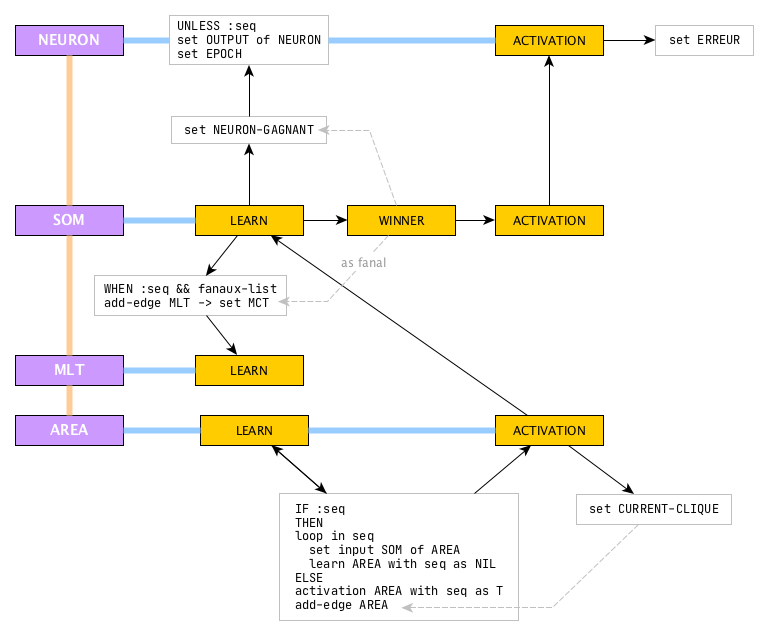
\includegraphics[width=\columnwidth]{4356}
\caption[Summary of the learning process in N3.]{Summary of the learning process in N3\protect\footnotemark.}
\label{fig:resn3}
\end{center}
\end{figure}

\footnotetext{\begin{itemize}
\item[$\bullet$] The learning is dependant of the encoding in relation to the desired environment or the kind of required `control'.
\item[$\bullet$]  Each sequence is identified upstream and downstream by a `\textit{tout-à-zéro}' marker. 
\item[$\bullet$]  The learning at the AREA level consists to activate the current clique (via \textit{microcolonnes} activation) in order to record it as arcs. At the same time, each MLT records arcs and \textit{tournois} connected to the previous clique. 
\end{itemize}}

